\documentclass[xcolor=dvipsnames]{beamer} % dvipsnames gives more built-in colors
\usetheme{Madrid}
%\useoutertheme{miniframes} % Alternatively: miniframes, infolines, split
\useinnertheme{circles}



%Define the colurs
%\definecolor{DarkMagenta}{rgb}{0.369, 0, 0.49}
%\definecolor{StrongMagenta}{rgb}{0.702, 0, 0.702}
%\definecolor{PaleViolet}{rgb}{0.918, 0.749, 1.000}
%\definecolor{VeryLightViolet}{rgb}{0.835, 0.502, 1.000}
\definecolor{Champagne}{rgb}{0.992, 0.922, 0.75}
\definecolor{RoseQuartz}{rgb}{0.953, 0.723, 0.719}
\definecolor{BlueGray}{rgb}{0.332, 0.406, 0.563}
\definecolor{Black}{rgb}{0.121, 0.125, 0.125}

%Instead of using \usecolortheme define yours
\setbeamercolor{palette primary}{bg=RoseQuartz,fg=BlueGray}
\setbeamercolor{palette secondary}{bg=Champagne,fg=Black}
\setbeamercolor{palette tertiary}{bg=BlueGray,fg=white}

%Title page things
\setbeamercolor{title}{bg=RoseQuartz,fg=Black}
\title[Heuristics for Weighted Graph Bandwidth]{\textbf{Heuristic Bandwidth Reduction Algorithms for Weighted Graphs}}
\author[Luis M. B. Varona]{\emph{Luis M. B. Varona}\inst{1,2,3}} 
\institute[MtA]{\small Joint Work with \emph{Alexander Matheson}\inst{2}} 
\date[July 24, 2026]{East Coast Combinatorics Conference 2026}
\titlegraphic{
\includegraphics[width=4cm]{assets/mta-logo.png}} 
\setbeamertemplate{navigation symbols}{} %For clearing the symbols at the bottom


%Itemize color and shape change
\setbeamertemplate{itemize item}[circle]
\setbeamertemplate{itemize subitem}[circle]
\setbeamercolor{itemize item}{fg=BlueGray}
\setbeamercolor{itemize subitem}{fg=BlueGray}

%Frame Title Change
\setbeamercolor{frametitle}{fg=Black,bg=RoseQuartz}
\setbeamerfont{frametitle}{series=\bfseries,parent=structure}

%Theorems and blocks
\setbeamercolor{block title}{use=structure,fg=Black,bg=RoseQuartz}
\setbeamercolor{block body}{use=structure,fg=black,bg=white}
\addtobeamertemplate{block begin}{%
		\setlength{\textwidth}{0.9\textwidth}%
}{}



\usepackage{ragged2e} %For justifying the text
\justifying

\usepackage[skins,theorems]{tcolorbox} %colored boxes for equations
\tcbset{highlight math style={enhanced,colframe=Black,colback=white,arc=0pt,boxrule=1pt}}


\usepackage{amssymb} %Symbols from the American Mathemetical Society
\usepackage{amsmath} %Equations
\usepackage{mathtools} %Extention to amsmath
\usepackage{mathrsfs} %For curly L in Cartan's equation
\usepackage{dsfont}
\usepackage{physics} %For abs

\usepackage{caption} %for captions


\setbeamerfont{footnote}{size=\tiny}

\definecolor{DeepBlue}{rgb}{0.0, 0.2, 0.4}

% nice-looking footnotes in slides
\usepackage[absolute,overlay]{textpos}
\newenvironment{reference}[2]{%
  \begin{textblock*}{\textwidth}(#1,#2)
  \footnotesize\it\bgroup\color{DeepBlue}}{\egroup
\end{textblock*}}

\newcommand{\bij}{%
  \hookrightarrow\mathrel{\mspace{-15mu}}\rightarrow
}

\makeatletter
\newcommand{\xbij}[2][]{%
  \lhook\joinrel
  \ext@arrow 0359\rightarrowfill@ {#1}{#2}%
  \mathrel{\mspace{-15mu}}\rightarrow
}
\makeatother

\def\I{\mathbb{1}}
\def\O{\mathbb{O}}
\def\C{\mathbb{C}}
\def\N{\mathbb{N}}
\def\Z{\mathbb{Z}}
\def\Q{\mathbb{Q}}
\def\R{\mathbb{R}}
\def\E{\mathbb{E}}
\def\F{\mathbb{F}}

\def\B{\mathcal{B}}
\def\D{\mathcal{D}}
\def\Ein{\mathcal{E}}
\def\K{\mathcal{K}}
\def\Lin{\mathcal{L}}
\def\M{\mathcal{M}}
\def\S{\mathcal{S}}
\def\U{\mathcal{U}}
\def\V{\mathcal{V}}
\def\W{\mathcal{W}}
\def\X{\mathcal{X}}
\def\Y{\mathcal{Y}}

\def\a{\mathbf{a}}
\def\b{\mathbf{b}}
\def\c{\mathbf{c}}
\def\d{\mathbf{d}}
\def\e{\mathbf{e}}
\def\p{\mathbf{p}}
\def\q{\mathbf{q}}
\def\r{\mathbf{r}}
\def\u{\mathbf{u}}
\def\vv{\mathbf{v}} % To avoid overriding `\v` (caron diacritic)
\def\w{\mathbf{w}}
\def\x{\mathbf{x}}
\def\y{\mathbf{y}}
\def\z{\mathbf{z}}
\def\0{\mathbf{0}}
\def\1{\mathbf{1}}

\renewcommand{\emph}[1]{\textcolor{Blue}{\textbf{#1}}}


\begin{document}

{
    \setbeamertemplate{footline}{} %deleting the slide number from the title page
    \begin{frame}
        \vspace*{-0.8cm}
        \titlepage
        \begin{reference}{10mm}{83mm}
            \rule{4cm}{0.5pt} \\
            \scriptsize
            \textsuperscript{1}Department of Politics \& International Relations, Mount Allison University \\
            \textsuperscript{2}Department of Mathematics \& Computer Science, Mount Allison University \\
            \textsuperscript{3}Department of Economics, Mount Allison University \par
        \end{reference}
    \end{frame}
}
\addtocounter{framenumber}{-1}	%resetting the counting for the slides

\begin{frame}
    \frametitle{\normalfont Graph Bandwidth and Applications}
    \begin{itemize}
        \item \emph{Layout} of $G$: a bijection $\pi : V(G) \to \bigl\{0, 1, \ldots, \bigl\lvert V(G) \bigr\rvert - 1\bigr\}$ \vfill
        \item \emph{Bandwidth} of $G$ under layout $\pi$: $\beta_{\pi}(G) = \max\limits_{\{u, v\} \in E(G)} \bigl\lvert \pi(u) - \pi(v) \bigr\rvert$ \vfill
        \item Interested in finding \emph{low-bandwidth layouts} because of applications in optimizing circuit layout, speeding up PDE solvers, etc. \vfill
        \item e.g., paths have \emph{minimum bandwidth} $\beta(P_n) = 1$, stars have $\beta(S_n) = \lfloor n / 2 \rfloor$, and complete graphs have $\beta(K_n) = n - 1$  \vfill
        \item For a \emph{weighted graph}: $\beta_{\pi}(G) = \max\limits_{\{u, v\} \in E(G)} w(u, v) \cdot \bigl\lvert \pi(u) - \pi(v) \bigr\rvert$, where $w$ is the weight function \vfill
        \item Most algorithms are for unweighted graphs only; these neglect, e.g., non-uniform \emph{timing criticality} when designing circuits \vfill
    \end{itemize}
\end{frame}

\begin{frame}
    \frametitle{{\normalfont Designing Algorithms for Weighted Bandwidth}}
    \begin{itemize}
        \item \emph{Reverse Cuthill--McKee} (RCM) and other heuristics \textit{can} be trivially adapted to weighted graphs, but this is rather suboptimal \vfill
        \item My (very early-stages) \emph{``Big Bear 1011''} algorithm: \vfill
        \begin{enumerate}
            \item Takes a linear forest with high-weight edges, then contracts all paths (computing the weights of the new edges is nontrivial) \vfill
            \item Runs both weighted RCM and a custom RCM where all edges below a certain weight threshold are (temporarily) deleted \vfill
            \item Re-expands the super-nodes and returns the better layout \vfill
        \end{enumerate} \vfill
        \item Rmk.: Custom RCM wins on ``heavy-backbone'' graphs (e.g., \emph{VLSI circuits} or \emph{caterpillars}); weighted wins on fairly uniform graphs \vfill
    \end{itemize}
    
\includegraphics[height=1.8cm]{assets/pusheen-reading.png}
\end{frame}

\begin{frame}
    \frametitle{Observe: {\normalfont Big Bear in Action!}}
    {
        \setbeamerfont{caption}{size=\scriptsize}
        \setlength{\belowcaptionskip}{-3.65pt}
        \begin{figure}
            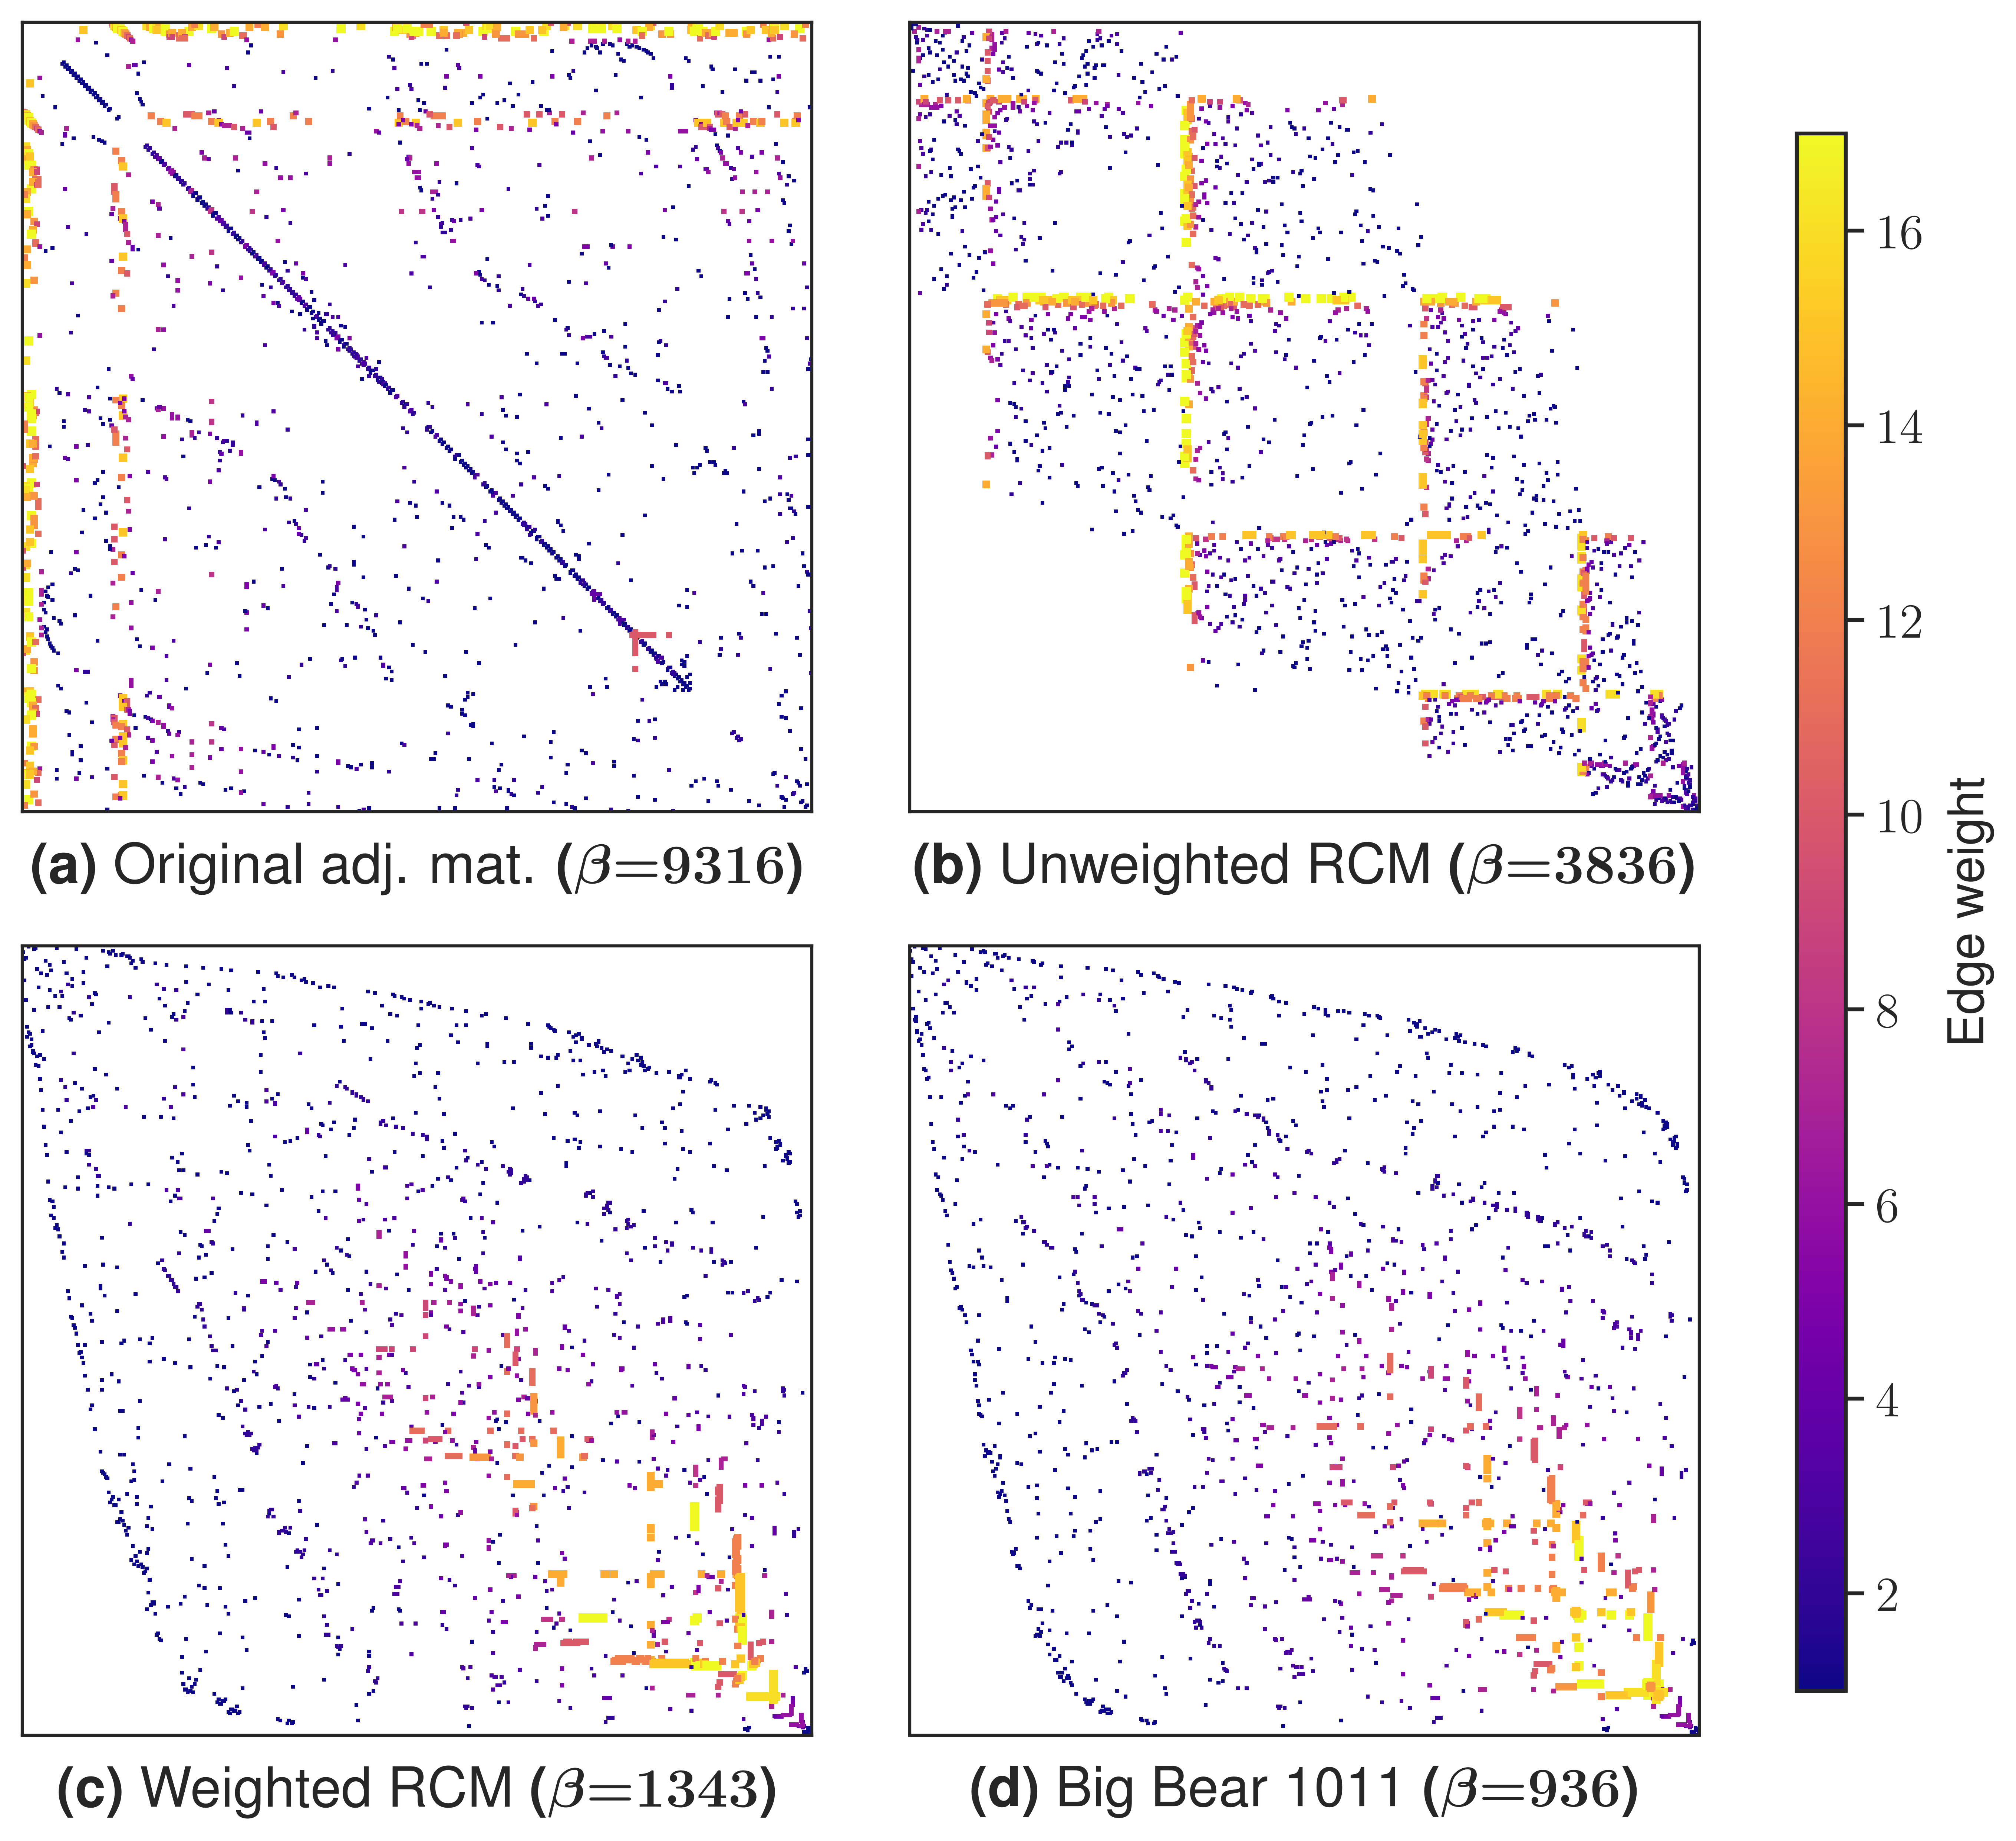
\includegraphics[height=7cm]{assets/iscas89_s1196_weighted_bw.png}
            \caption{``Big Bear 1011'' reduces $\beta$ by $\mathord{>} 30\%$ more than weighted RCM on a \emph{$561$-cell circuit} benchmark (s1196, ISCAS 1989). [Code: \href{https://doi.org/10.5281/zenodo.21483800}{\textcolor{purple}{github.com/Luis-Varona/eccc-2026-weighted-bw}}.]}
        \end{figure}
    }
\end{frame}

\end{document}
